%
%  Vincent Yannello
%
\documentclass[12pt,fullpage]{article}
\usepackage{fullpage}
\usepackage{psfrag}                                          % LaTeX graphics tool
\usepackage{pslatex}                                         % avoids the default cmr font
\usepackage{graphicx}                                        % graphics package 
\usepackage{epsfig}
\usepackage{hyperref}
\usepackage{color}

\begin{document}

\noindent
{\bf Beta--Pascal distribution} (from \color{blue}\url{http://www.math.wm.edu/~leemis/chart/UDR/UDR.html}\color{black})

\noindent
The shorthand $X \sim {\rm betapascal}(n, a, b)$ is used to indicate that the
random variable $X$ has the beta--pascal distribution with parameters $n$, $a$, and $b$.
A beta--Pascal random variable $X$ with parameters~$a,~b,$ and $n$ has probability mass function 
$$
f(x) = \frac {{n-1+x\choose x} B  \left( n+a, \, b+x \right) }{
B \left( a, \, b \right) } \quad \quad x = 0, 1, \ldots \ .
$$
A beta--Pascal random variable is a Pascal random variable with a random parameter $p$ which has the
beta distribution with parameters $a$ and $b$.
The probability mass function for $n=10$ and three different parameter settings is illustrated below. \\

\begin{figure}[h!]
\begin{center}
\psfrag{labx}{$x$}
\psfrag{labf}{$f(x)$}
\psfrag{laba1}{$a = 1$}
\psfrag{laba2}{$a = 2$}
\psfrag{labb1}{$b = 1$}
\psfrag{labb2}{$b = 2$}
\includegraphics[width=5.6in]{BetapascalPlot.ps}
\end{center}
\end{figure}

\noindent
The cumulative distribution function on the support of X is
$$
F(X) = P(X \leq x) = \displaystyle \sum_{w=0}^x \frac {{n-1+w\choose w} B  \left( n+a, \, b+w \right) }{
B \left( a, \, b \right) } \quad \quad x = 0, 1, \ldots \ .
$$
The survivor function on the support of X is
$$
S(X) = P(X \geq x) = \displaystyle \sum_{w=x}^\infty \frac {{n-1+w\choose w} B  \left( n+a, \, b+w \right) }{
B \left( a, \, b \right) } \quad \quad x = 0, 1, \ldots \ .
$$
for all $a>0$, $b>0$, and $n= 1, 2, \ldots.$ The hazard function,
cumulative hazard function, inverse distribution function, moment generating function, and characteristic function 
on the support of $X$ are all mathematically intractable.

\vspace{0.05in}

\noindent
The population mean, variance, skewness, and kurtosis of $X$ are all mathematically intractable.

\newpage

\noindent
{\bf APPL verification:}
The APPL statements
\begin{verbatim}
assume(a > 0);
assume(b > 0);
X :=[[x -> binomial(n - 1 + x, x) * Beta(n + a, b + x) / Beta(a, b)],
     [0 .. infinity], ["Discrete", "PDF"]];
CDF(X);
SF(X);
HF(X);
CHF(X);
Mean(X);
Variance(X);
Skewness(X);
Kurtosis(X);
MGF(X);
\end{verbatim}
verify the cumulative distribution function, survivor function, hazard function, cumulative hazard function,
and inverse distribution function, but fail to yield moment generating function or the expected values beyond the general definition.

\end{document}
